%======================================================================
\section{Physical Unclonable Functions - PUFs}
\label{sec:pufs}
\pufs~are physical functions created to mimic random functions. Their inputs, called challenges, and outputs, called responses, are designed to have a unique relation for every \puf~instance. This is achieved by leveraging on imperfections resulted from fabricating electronic devices.

\subsection{PUF types}
\begin{figure*}[!ht]
	\centering
% 	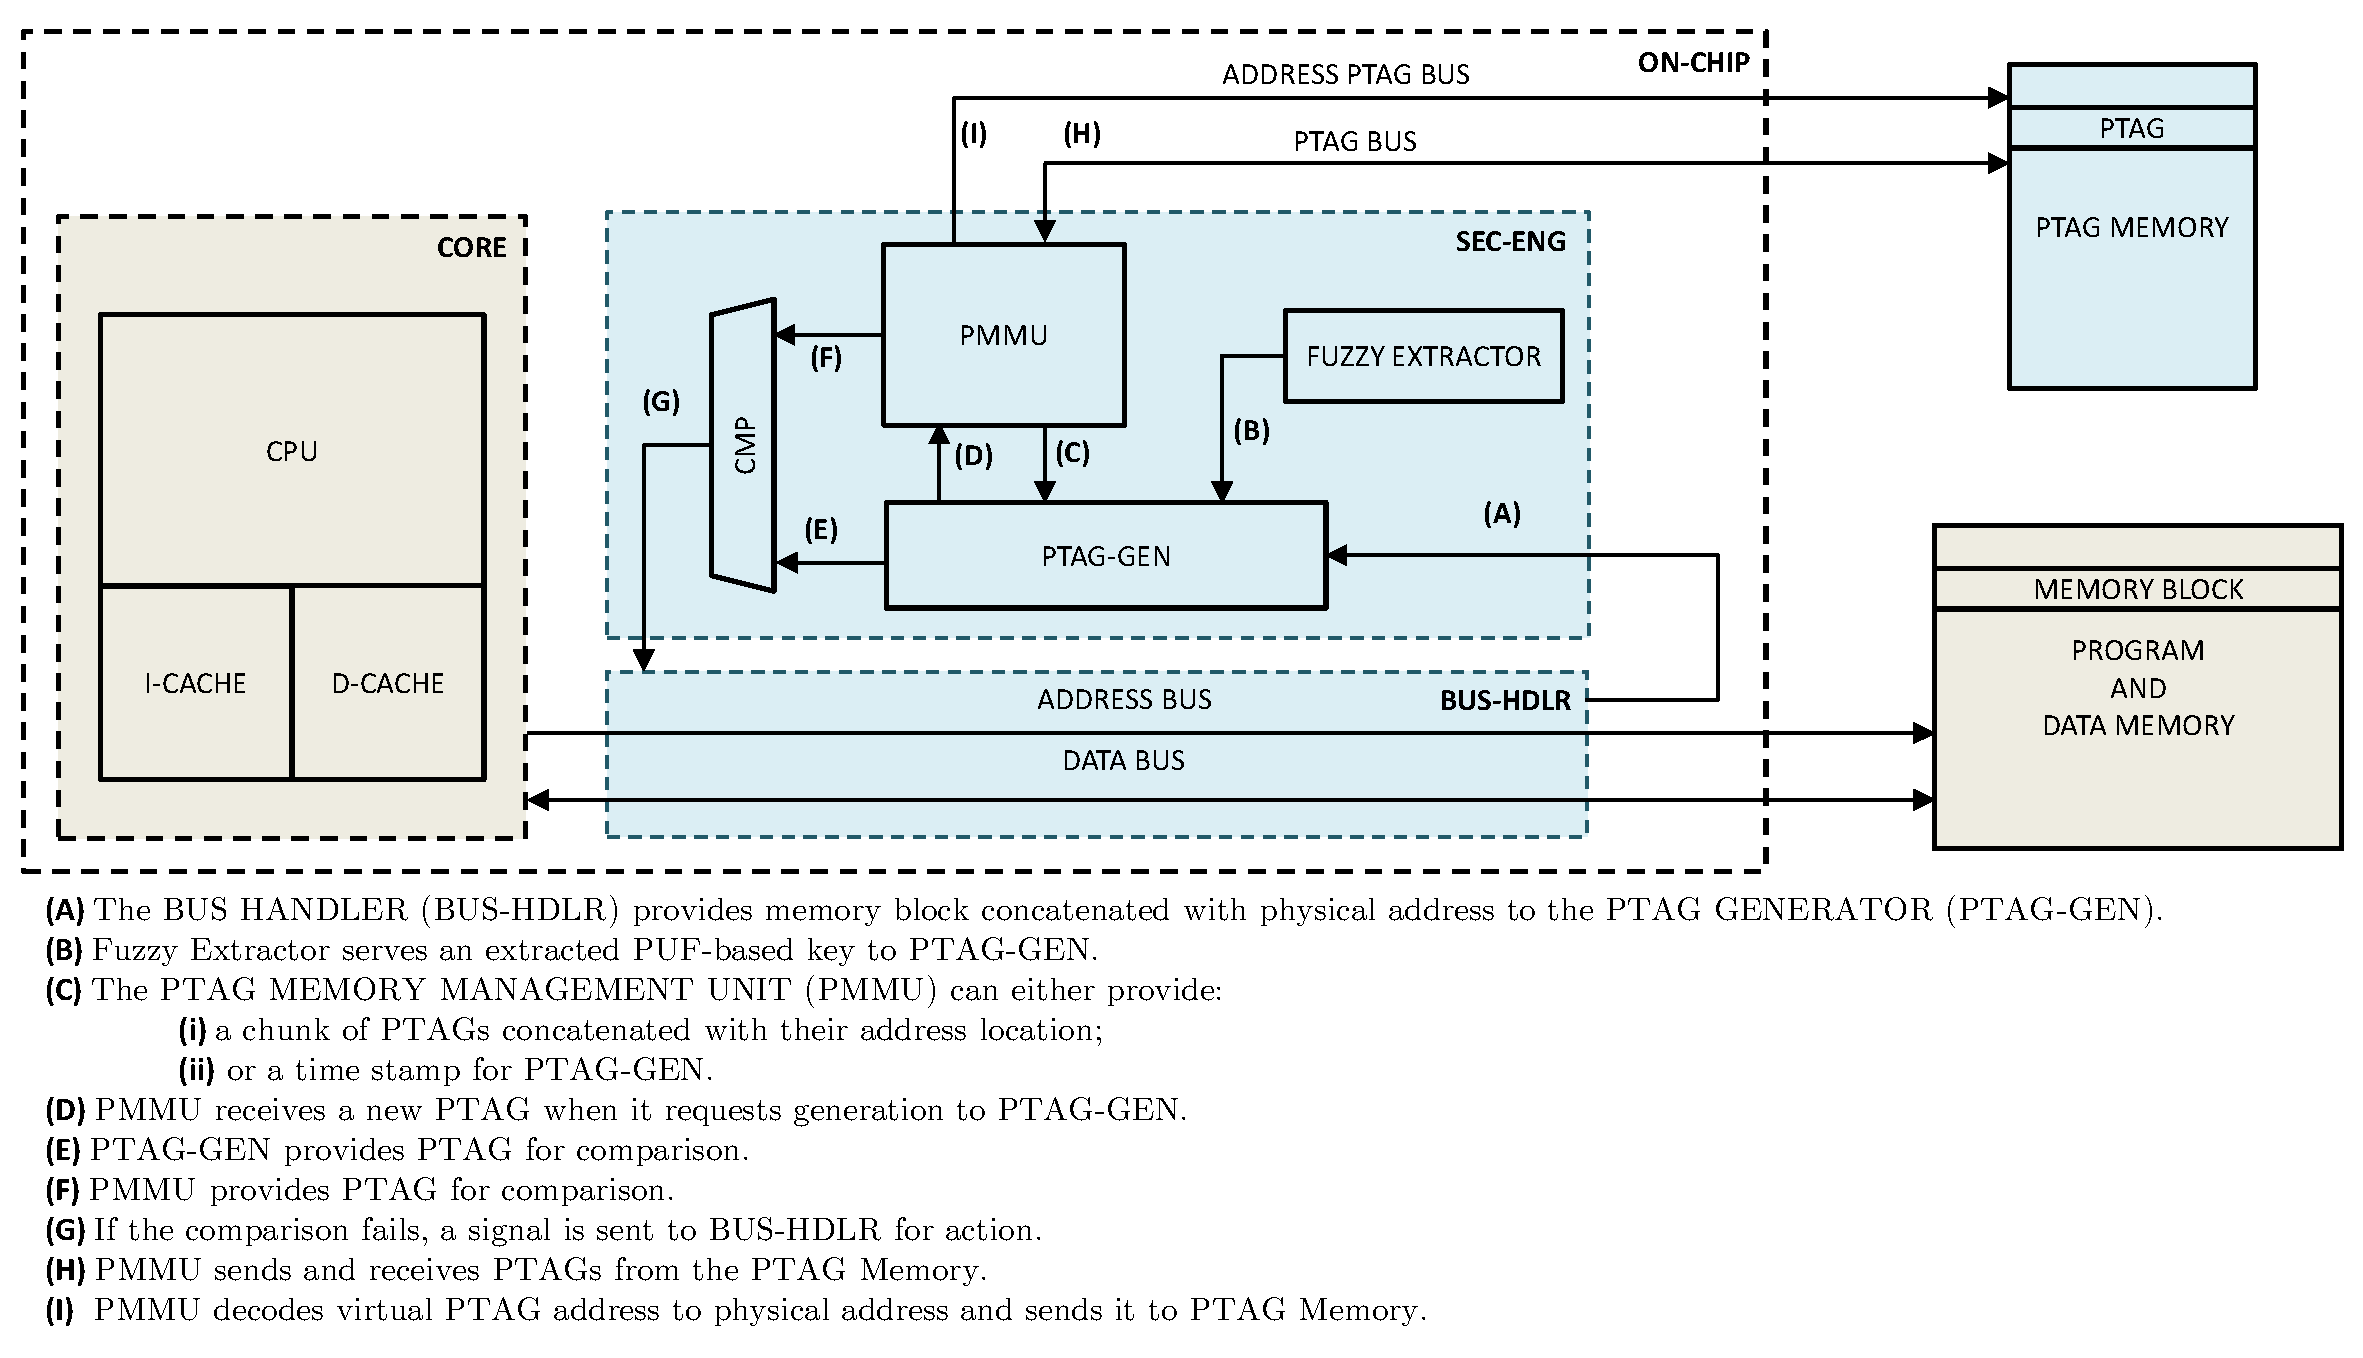
\includegraphics[scale=0.45]{cshia}
	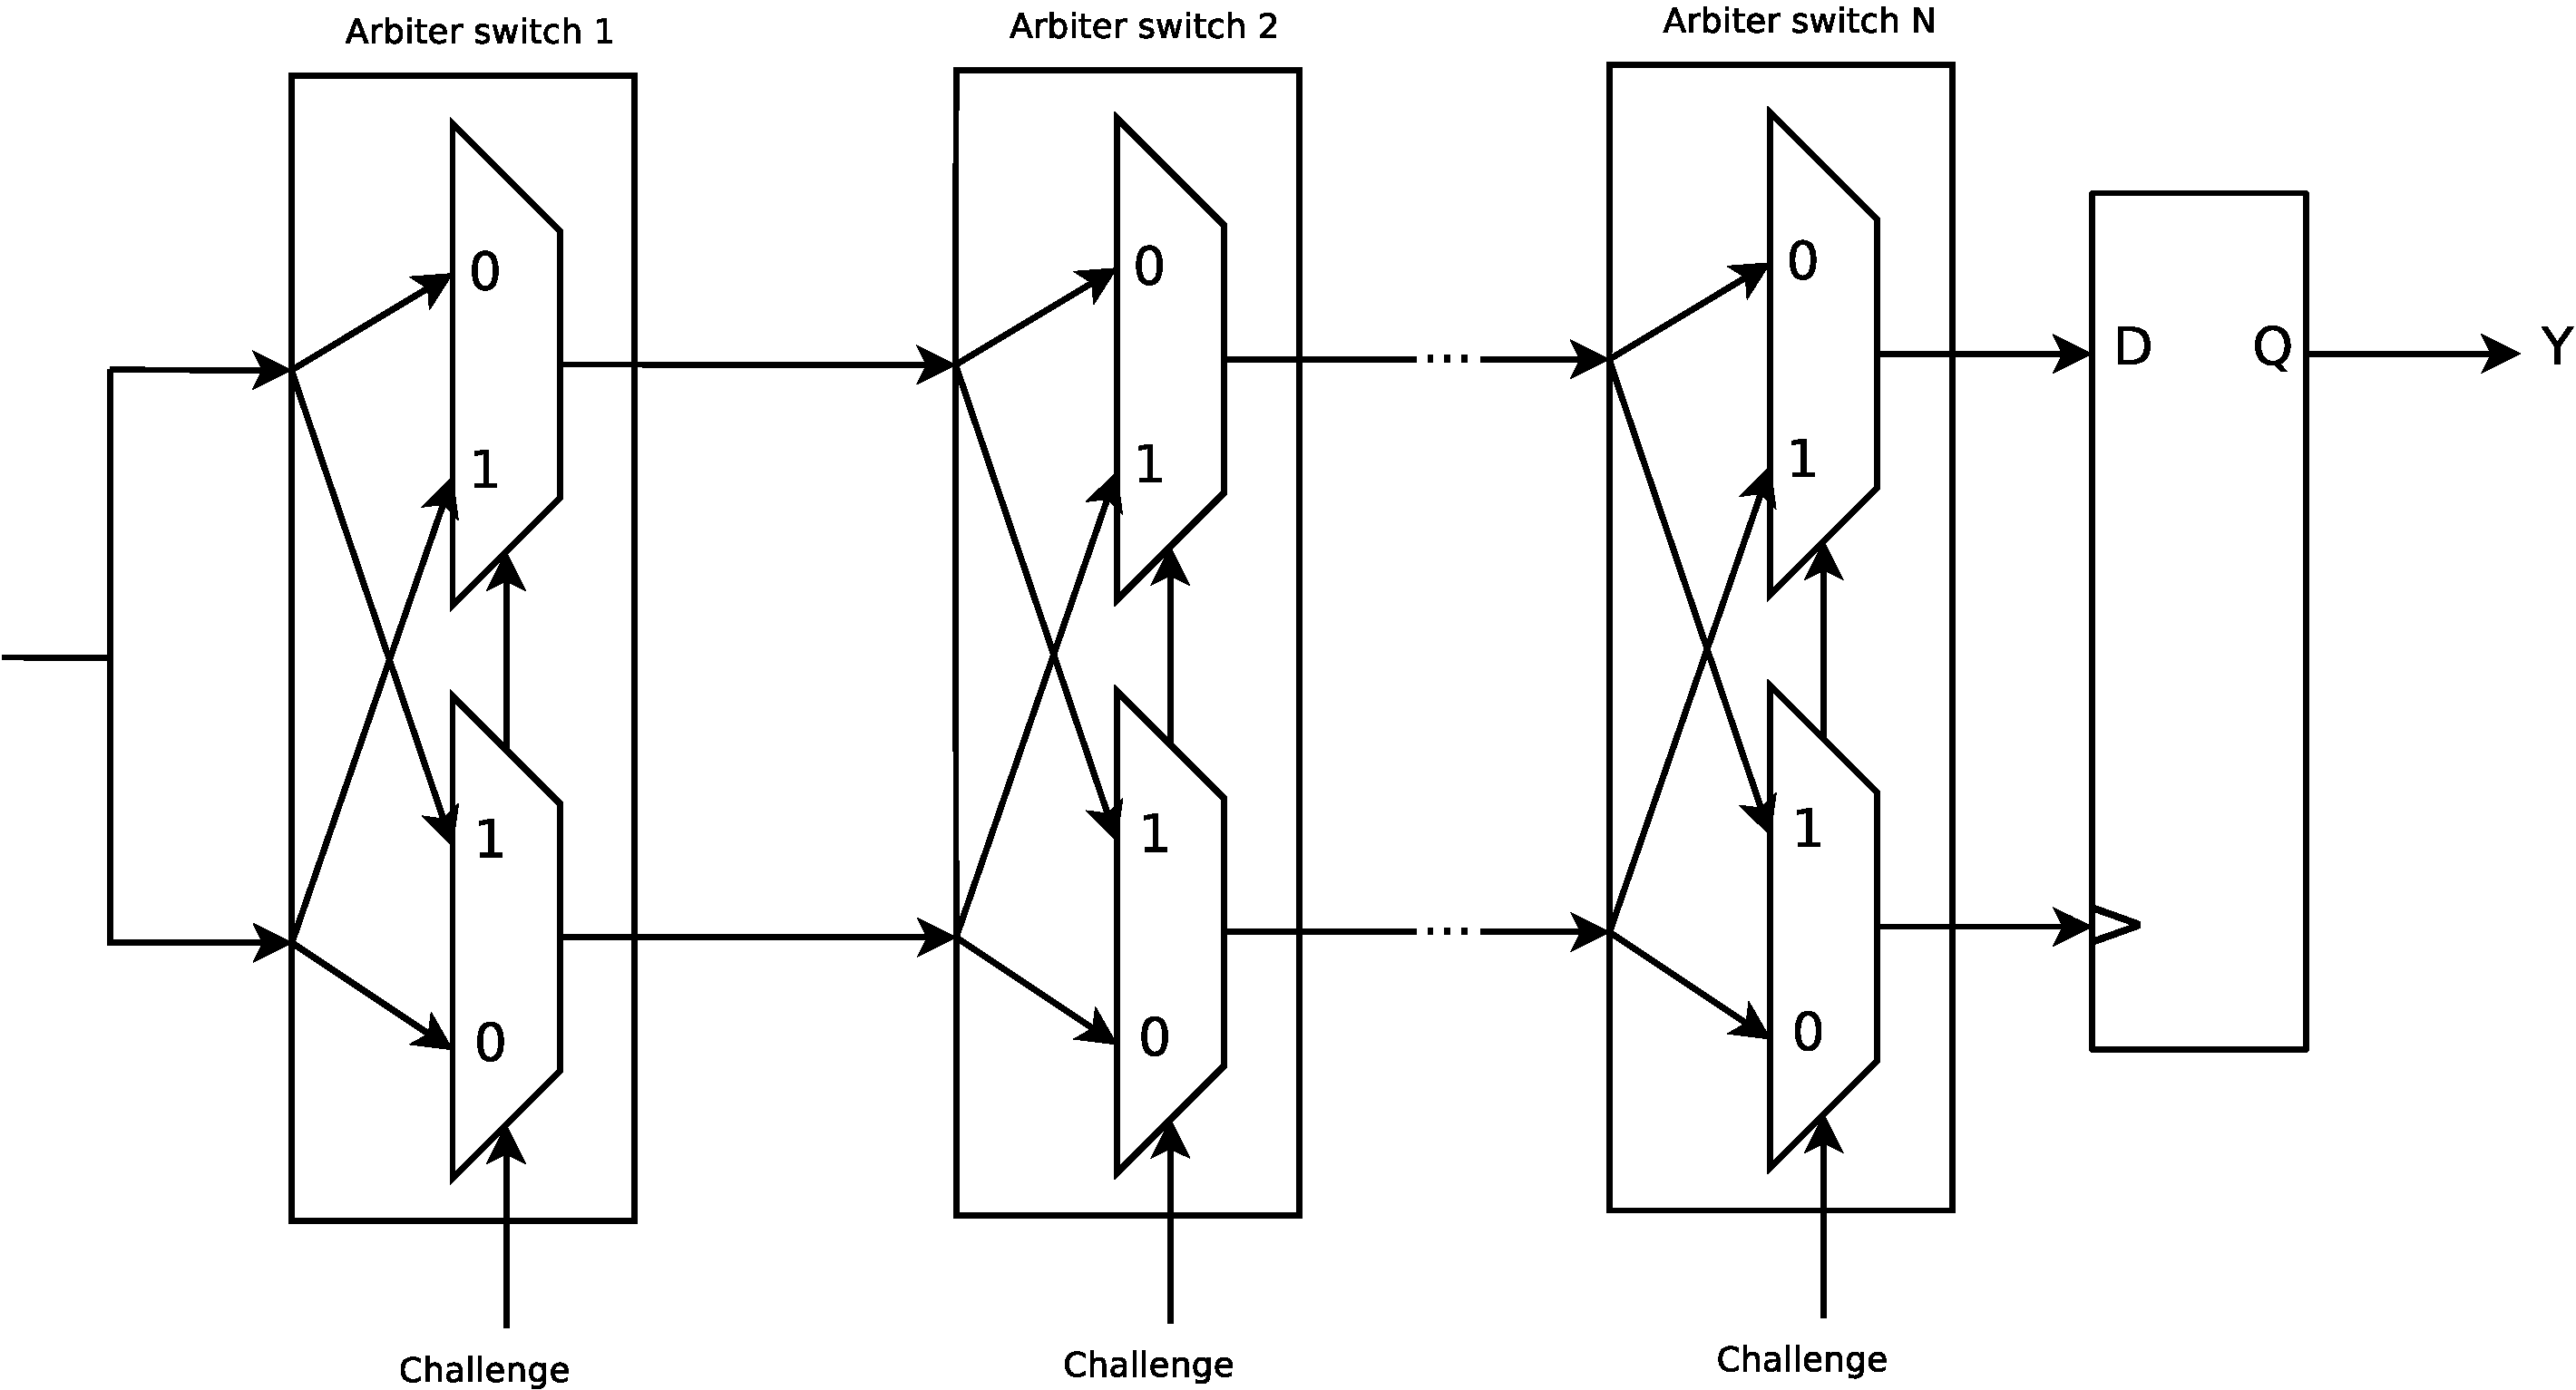
\includegraphics[width=\textwidth]{arbiter}
	\caption{The \cshia~architecture.}
%	\vspace*{-9pt} 
	\label{fig:cshia}
\end{figure*}

\subsection{PUF as a key}
When a system needs a key in hardware for any purpose, such as encryption, authentication or any other application, this key needs to be generated  and stored in hardware
\cite{puf-key-devadas-1278484}. The main advantage of using \pufs~as key generators is that they can produce keys at running time, this way, on-chip memories are not needed for key storage. Another benefit is that they are unclonable, meaning that even the manufacturer itself cannot produce two \puf~instances that will have the same set of Challenge-Response Pairs (\crps) \cite{Gassend2002:PUFs}.


%======================================================================
\section{Security Properties}
\label{sec:securityproperties}
In order to counter the attacks discussed above, a system designer need to employ mechanisms that implements three security properties: authenticity, integrity, and secrecy. Although these features can be implemented through software, the stringent nature of embedded systems demands solutions that consume few clock cycles and are not power consuming.
In the following, we discuss hardware implementation of those security features.

%---------------------------------------------------------
\subsection{Authenticity}
\label{subsec:Authenticity}
Suppose that an attacker wants to add \hisher~own code for execution in the embedded system or intends to move the data from one system instance to another. These attacks can be avoided by employing authentication mechanisms. In this solution, a key (or unique set of keys) is determined for each instance.
%TODO explain the instance more clear
Code \andor~ data are tagged using these keys during manufacturing (an enrollment phase). At run time, this key (or set of keys) is used to regenerate tags. Only a correct key value will be able to verify what was installed during manufacture. Therefore, an instance will not accept code or data that was not tagged using its own keys.

Before the introduction of electronic \pufs \cite{Gassend2002:PUFs}, these keys had to be inserted into the system  before they were made available to the users. To do so, keys are stored on chip using non-volatile memories and the manufacturer\slash{}vendor controlled the uniqueness of the keys in each instance. The main downsides of storing key permanently include: facilitating physical attacks \cite{Sadeghi2010:Security-PUFs}, and possibly increasing costs of production since it may demand integration of different technologies on the same chip.

%---------------------------------------------------------
\subsection{Integrity}
\label{subsec:integrity}
\ref{subsec:integrity}
Similarly  to authentication, integrity is ensured by tagging code and data with additional information such as memory address location \andor~timestamps. This prevents an attacker from tampering with a system by, for instance, moving instructions from their location in memory, setting different initial values of variables, etc. The level of integrity can be done for an entire program, memory pages, or memory blocks. 

Integrity can also be considered at the instruction sequence level, which we refer as Control-Flow Integrity (CFI). Hardware solutions for control-flow integrity usually require deep integration between hardware and software \cite{Davi2015:HAFIX}, that can result not only in changing the Instruction Set Architecture (\isa) \andor~the tool-chain, but also the processor's data path, as proposed in \cite{Gelbart2005:CODESSEAL, Kanuparthi2012:DynamicIntegrity}. Even though CFI protection is welcomed, many embedded system applications cannot afford the performance penalties and storage overhead inherently of this solution. For instance, in applications where user inputs are limited and \io~involves fixed amounts of data, an attacker has very little room to employ a buffer overflow or similar attacks prevented by CFI. However, integrity verification regarding blocks of code and data (as mentioned above) can avoid a variety of situations that go beyond run time attacks. For example, if an embedded system is unwatched, an attacker can upload a malicious code or modify the data in the external memory even if the system is not running. Integrity verification can prevent and indicate these violations before they reach the processor.


%---------------------------------------------------------
\subsection{Secrecy}
\label{subsec:Secrecy}

An embedded system can also use encryption to prevent exposure of code \andor~data stored in the external memory. Consequently, the processor can run these instructions and data only after decryption. Therefore, the major drawback of using encryption is the performance overhead that highly depends on which cryptographic primitive is employed \cite{Suh2007:PUFs}. In addition, secrecy only prevents that an attacker obtains the information, if it is not combined with a unique key or integrity verification, the system will be vulnerable to execute code of different system instances \andor~to suffer relocation and replay attacks\cite{Elbaz2009}.